\section{Selected vertices, propagators, and regulator insertions}\label{app:GNvpr}
\renewcommand{\FSk}{t}
In this appendix we will present the for \cref{chap:GN} relevant two-point functions, regulator insertions, propagators, and vertices. 
Those are obtained by taking functional derivatives of the \eaa{} \eqref{eq:gnyLPAansatz} and the corresponding, canonical regulator term \eqref{eq:DeltaSRab} and evaluating the resulting expressions on the \qeom{}, \viz{} projecting on to $\FSsfEoM{}=\MFEchi{}\equiv(\sigma,0,0)$ from \cref{eq:GNYVEV}:
\begin{align}
\big(A_{\ldots}^{\ldots}\big)_{\chi=\FSsfEoM{}=\MFEchi{}}\equiv \underline{A}_{\ldots}^{\ldots}\,.
\end{align}
We will mark uncontracted, external indices with an underscore, in the spirit of \cref{subsec:higherOrderFlowEquations}.
We will use $f$ as flavor index and $a$ for spinor indices.

This appendix has a corresponding digital auxiliary file~\cite{Steil:2023GNnotebook}.\bigskip

The non-vanishing two-point functions are
\begin{subequations}\label{eq:GNGamma2}
\begin{alignat}{2}
\FSvertexArg{\FSeaaEoM}{\MFpsib_{\iEI}, \MFpsi^{\iEII}}&\equiv\begin{gathered}\raisebox{-3pt}{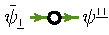
\includegraphics{appendix/diagrams/GN2-Gamma2tbt.pdf}}\end{gathered}&&= -\deltapnS[p_\iEI-p_\iEII][1][n_\iEI-n_\iEII] (\Id_N)^{f_\iEI}{}_{f_\iEII}\big(\iu(\nu_{n_\iEI}+\iu \mu)\gamma^2+\iu p_\iEI\gamma^1+\tfrac{h \sigma}{\sqrt{N}}\Id_2\big)^{a_\iEI}{}_{a_\iEII}\,,\\
\FSvertexArg{\FSeaaEoM}{\sigma_{\iEI},\sigma_{\iEII}}&\equiv \begin{gathered}\raisebox{-3pt}{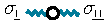
\includegraphics{appendix/diagrams/GN2-Gamma2ss.pdf}}\end{gathered} &&= \deltapnS[p_\iEI+p_\iEII][1][n_\iEI+n_\iEII] \big(\omega_{n_\iEI}^2 +p_\iEI^2+\FScoupling{u}{1}{\sigma}\big) \,.
\end{alignat}
\end{subequations}

The regulator insertions are given by
\begin{subequations}\label{eq:GNdtR}
\begin{alignat}{2}
-\partial_t\FSregulatorArg{\FSREoM}{\MFpsib_{\iEII}, \MFpsi^{\iEI}}&\equiv\begin{gathered}\raisebox{-3pt}{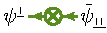
\includegraphics{appendix/diagrams/GN2-Rttb.pdf}}\end{gathered}&&= \deltapnS[p_\iEI-p_\iEII][1][n_\iEI-n_\iEII] (\Id_N)^{f_\iEI}{}_{f_\iEII}\big(\iu p_\iEI\gamma^1 \partial_t r_\mathrm{f}(t,p_\iEI)\big)^{a_\iEI}{}_{a_\iEII}\,,\\
\partial_t\FSregulatorArg{\FSREoM}{\sigma_{\iEI},\sigma_{\iEII}}&\equiv \begin{gathered}\raisebox{-3pt}{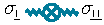
\includegraphics{appendix/diagrams/GN2-Rss.pdf}}\end{gathered} &&= \deltapnS[p_\iEI+p_\iEII][1][n_\iEI+n_\iEII] \big(\omega_{n_\iEI}^2 +p_\iEI^2 \partial_t r_\mathrm{b}(t,p_\iEI) \big) \,,
\end{alignat}
\end{subequations}
where we follow the diagrammatic conventions of \cref{app:SU2FSelements}, momentum-space conventions of \cref{app:fourier}, and only consider the one class of fermionic contributions and unify the other by means of transposition as discussed in \cref{app:SU2FSelements}.

The propagators are given by
\begin{subequations}\label{eq:GNG}
\begin{alignat}{2}
\FSpropagatorArg{\FSGEoM}{\MFpsi_{\iEI}, \MFpsib^{\iEII}} &=\begin{gathered}\raisebox{-3pt}{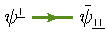
\includegraphics{appendix/diagrams/GN2-Gttb.pdf}}\end{gathered}&&= 
-\deltapnS[p_\iEI-p_\iEII][1][n_\iEI-n_\iEII] (\Id_N)^{f_\iEI}{}_{f_\iEII}\frac{\big(\iu(\nu_{n_\iEI}+\iu \mu)\gamma^2+\iu p_\iEI\gamma^1-\tfrac{h \sigma}{\sqrt{N}}\Id_2\big)^{a_\iEI}{}_{a_\iEII}}{(\nu_{n_\iEI}+\iu \mu)^2 +  p_{\iEI;k(t)}^2+ \tfrac{h^2 \sigma^2}{N} }\, ,\\
\FSpropagatorArg{\FSGEoM}{\sigma_{\iEI},\sigma_{\iEII}}&= \begin{gathered}\raisebox{-3pt}{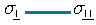
\includegraphics{appendix/diagrams/GN2-Gss.pdf}}\end{gathered} &&= \deltapnS[p_\iEI+p_\iEII][1][n_\iEI+n_\iEII] \frac{1}{\omega_{n_\iEI}^2 +p_{\iEI;k(t)}^2+\FScoupling{u}{1}{\sigma}}\,,
\end{alignat}
\end{subequations}
where we used the compact notation for the regulated spatial momenta $p_{;k}$ of \cref{eq:pkReg}.

For the flow equation discussed in \cref{app:GNtwopt} we additionally require the vertex
\begin{alignat}{2}
\FSvertexArg{\FSeaaEoM}{\MFpsib_{\iEI},\sigma_\iEII, \MFpsib^{\iEIII}}&\equiv\begin{gathered}\raisebox{-3pt}{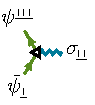
\includegraphics{appendix/diagrams/GN2-Vtbst.pdf}}\end{gathered}&&= \deltapnS[p_\iEII+p_\iEIII-p_\iEI][1][n_\iEII+n_\iEIII-n_\iEII] \tfrac{h}{\sqrt{N}} (\Id_2)^{a_\iEI}{}_{a_\iEIII}(\Id_N)^{f_\iEI}{}_{f_\iEIII}\,.
\end{alignat}

\section{The LPA flow equation}\label{app:GNlpa}
In this appendix we present a derivation of the \frg{} flow equation \eqref{eq:pdeq-U} of the effective potential $U ( t, \sigma )$ at non-zero $\mu$ and $T$ in \lpa{} truncation  for the sake of completeness. 
Tracing the \frgEq{} in field space using the propagators and regulator insertions of \cref{app:GNvpr} and projecting onto $\FSsfEoM{}=\MFEchi{}=(\sigma,0,0)$, \cf{} \cref{eq:GNYVEV}, yields
\begin{align}
	\beta ( 2 \piu ) \, \delta ( 0 ) \, \partial_t U ( t, \sigma ) &= \partial_t\FSvertexArg{\FSeaaEoM}{}	= 
	\frac{1}{2}\,\begin{gathered}
\includegraphics{gn/diagrams/GN2-UFlow2.pdf}\end{gathered} -\,\begin{gathered}
\includegraphics{gn/diagrams/GN2-UFlow1.pdf}\end{gathered}\, ,\label{eq:wetterich_background_field}
\end{align}
with an infinite volume factor $V\equiv \beta ( 2 \piu ) \, \delta ( 0 )$, which also appears in the loops on the \rhs{} and thus ultimately cancels.
Plugging in the explicit expressions of \cref{app:GNvpr}, we can perform the traces in Dirac and flavor space and are left with the traces in momentum space with manifest as one-dimensional momentum-space integrals and Matsubara sums. The flow equation ultimately reads
\begin{align}
	\partial_t U ( t, \sigma ) =& \frac{1}{2}\sumintpnS[p][][n][] \, \frac{p^2 \, \partial_t r ( t, p )}{\omega_n^2 + p^2 [ 1 + r ( t, p ) ] + \partial_\sigma^2 U ( t, \sigma )}\, -\nonumber\\
	&\qquad \qquad \qquad  - \sumintpnS[p][][n][] \, \frac{N \, p^2 \, \partial_t r ( t, p )}{ ( \nu_n + \iu \mu )^2 + p^2 [ 1 + r ( t, p ) ] + \frac{( h \, \sigma )^2}{N} } \,,		\label{eq:flow_equation_after_traces}
\end{align}
where we assumed a unified scheme for the regulator shape functions, according to \cref{eq:rfrbDef}:
\begin{align}
r( t, p )+1\equiv \rb( t, p )+1\equiv(\rf( t, p )+1)^2 \, .\label{eq:gnregs}
\end{align}
With the flat (\lpa{} optimized Litim) regulator shape function \eqref{eq:rflat} the momentum integral can be evaluated analytically, see, \eg{}, \ccite{Stoll:2021ori,Steil:2023GNnotebook} for the involved subtleties, and we arrive at
\begin{align}
	\partial_t U ( t, \sigma ) = \, & - \frac{1}{\piu} \, \frac{1}{\beta} \sum_n \, \frac{k^3 ( t )}{\omega_n^2 + E_\mathrm{b}^2 ( t, \sigma )} + \frac{2 N}{\piu} \, \frac{1}{\beta} \sum_n \frac{k^3 ( t )}{ ( \nu_n + \iu \mu )^2 + E_\mathrm{f}^2 ( t, \sigma )}\, .
\end{align}
The Matsubara sums can be evaluated analytically, as discussed in \cref{app:matsubaraSums}. The relevant expressions for this case are given in \cref{eq:Mb1,eq:Mf1}.
After the $\tfrac{1}{N}$-rescalings of \cref{eq:rescaling_with_n} we finally obtain \frg{} flow equation \eqref{eq:pdeq-U} for the scale-dependent effective potential in \lpa{} at non-zero $T$ and non-zero $\mu$.\bigskip
	
The corresponding expression in the large-$N$ limit with the sharp regulator shape function of \cref{eq:rsharp} relevant for some specifics of the discussion in \cref{sec:gnInfInhomo} will be included in \nbccite{Steil:2023GNnotebook}.

\section{The bosonic two-point function in the limit \texorpdfstring{$N\rightarrow\infty$}{ of infinite N}}\label{app:GNtwopt}
The bosonic two-point function discussed in the stability analysis of \cref{eq:gtwo_renorm} can be computed from the flow equation
\begin{align}
 \partial_t \FSvertexArg{\FSeaaEoM}{\sigma_{\iEI}, \sigma_{\iEII}} = -\frac{1}{2}\,\begin{gathered}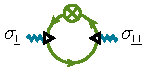
\includegraphics{gn/diagrams/GN2-TwoPtFlow1.pdf}\end{gathered}-\frac{1}{2}\,\begin{gathered}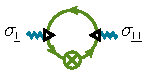
\includegraphics{gn/diagrams/GN2-TwoPtFlow2.pdf}\end{gathered}\, ,
\label{eq:gtwo_frg}
\end{align}
which in turn can be obtained by tracing \cref{eq:FS2} in field space with the expressions from \cref{app:GNvpr}.
Evaluating \cref{eq:gtwo_frg} at vanishing external frequency $n_\iEI=n_\iEII=0$ and external momenta $p_\iEI=-p_\iEII=q$ yields the required flow equation
$\partial_t\FSeaaEoM^{(2)}(\bar{\sigma},\mu,T,q)$, which can be integrated directly in the large-$N$ limit.
Choosing the sharp regulator shape function of \cref{eq:rsharp} or equivalently a sharp momentum cut-off in the unregularized variant of the flow equation, one can isolate the involved divergencies and equate them with the corresponding divergencies from the vacuum contribution. Careful consideration in a consistent regularization scheme allows for the computation of the renormalized result 
presented in \cref{eq:gtwo_renorm}. Additional details can be found in App.~A of \nbccite{Koenigstein:2021llr} and \ccite{Koenigstein:2022phd}.

\renewcommand{\FSk}{k}